
% #######################################################################################################################################
\chapter{Softmax Implementation}
\label{sec:Appendix-A}
\label{sec:Softmax Implementation}

In classifiers, the last layer is often implemented using a softmax \cite{wikipedia_softmax}\cite{stanford_softmax} function.
The outputs of this layer represent probabilities of each class/output.
As seen in Figure \ref{fig:classifier layer}, the classifier \ac{an} state calculation involves a \ac{mac} of the pre-synaptic \ac{an} states followed by an exponent.
The final \ac{an} state is the exponent of individual \acp{an} divided by the sum of all \acp{an} exponent value.

This work calculates the classifier \ac{an} states by separating the classifier into multiple layers as shown in Figure \ref{fig:classifier additional layers}.
The single classifier layer is implemented using three layers.
The first layer determines the exponent of each \ac{an}. This is accomplished using the \ac{stop} \ac{mac} operation followed by the \ac{simd} \ac{relu} and exponent \acp{sfu}.
The \ac{an} states of this layer are sent back to main memory.
The next layer is a single \ac{an} calculation, as described in Section \ref{sec:Processing a single ANe} with the pre-synaptic weights set to unity.
The resulting calculation is an accumulation of the \ac{an} exponent values.
The \ac{simd} divider \ac{sfu} is then used to perform a reciprocal and the result is placed in a \ac{simd} register.
The final layer is calculated using the \ac{stop} to perform a multiplication of each pre-synaptic \ac{an} state with the reciprocal value held in the \ac{simd} register, effectively performing the division in the softmax function.

Performing the softmax function is relatively inefficient, however the time taken is masked by the time taken to perform the initial classifier layer \ac{an} state calculation.
An example calculation sequence is shown in Figure \ref{fig:classifier implementation sequence timing} using the baseline \ac{ann} which employs one thousand classifiers with four thousand pre-synaptic \acp{an}.
\begin{figure}[h]
  \vspace{-5mm}
  \centering
  \captionsetup{justification=centering}
  \captionsetup{width=0.9\textwidth}
  \begin{minipage}{1\textwidth}
    \centering
    \centerline{
    \mbox{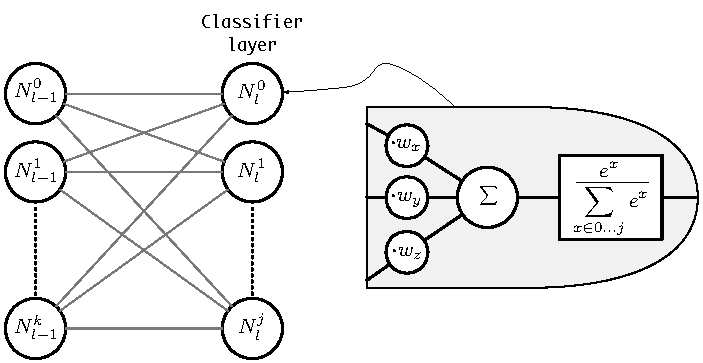
\includegraphics[angle=0, width=.65\textwidth]{classifierDiagram}}
    }
    \center\caption{Classifier layer}
    \label{fig:classifier layer}
  \end{minipage}
  \bigskip
  \vspace{-1mm}
  \begin{minipage}{1\textwidth}
    \centering
    \centerline{
    \mbox{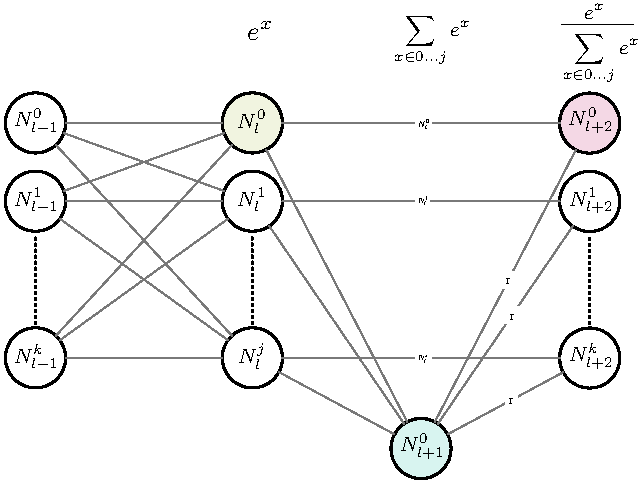
\includegraphics[angle=0, width=.55\textwidth]{classifierVirtualLayers}}
    }
    \caption{Classifier additional implementation layers}
    \label{fig:classifier additional layers}
  \end{minipage}
  %\captionof{figure}{Classifier}
  %\label{tab:Classifier}
\end{figure}

\newgeometry{margin=1in,lmargin=1.25in,footskip=\chapterfootskip}
\thispagestyle{lscapedlee}
\begin{landscape}
  \centering
  %\vspace*{\fill}
  \begin{figure}[h]
    \centering
    \vspace{0mm}
    \captionsetup{justification=centering}
    \captionsetup{width=0.9\linewidth}
    \begin{minipage}{1\linewidth}
      \centering
      \centerline{
      \mbox{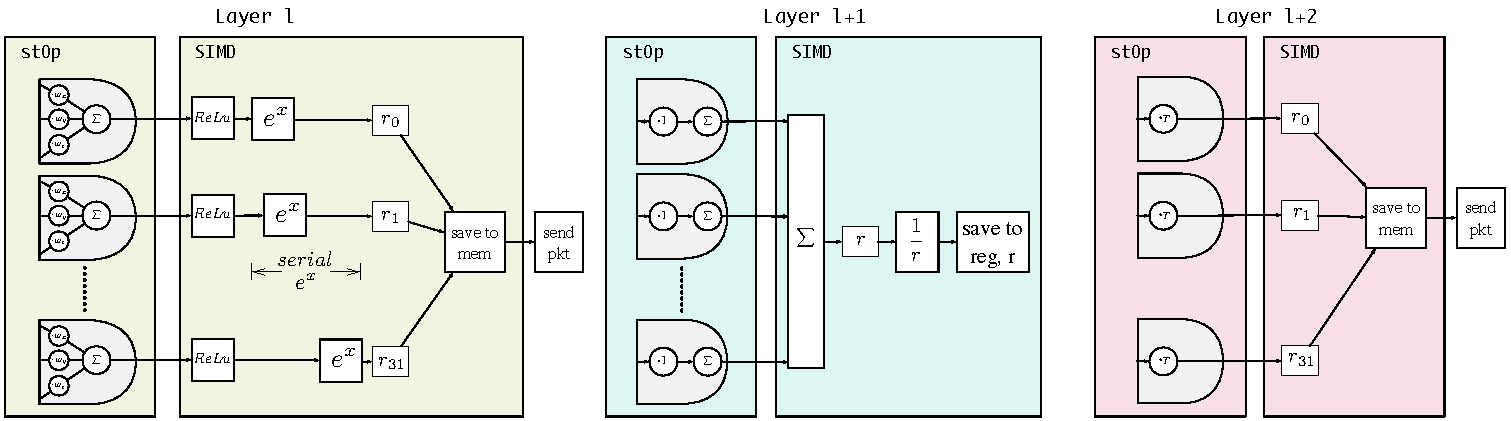
\includegraphics[angle=0, width=1\linewidth]{classifierImplementation}}
      }
      \caption{Classifier layer stOp/SIMD implementation}
      \label{fig:classifier implementation}
    \end{minipage}
    \bigskip
    \vspace{1mm}
    \begin{minipage}{1\linewidth}
      \centering
      \centerline{
      \mbox{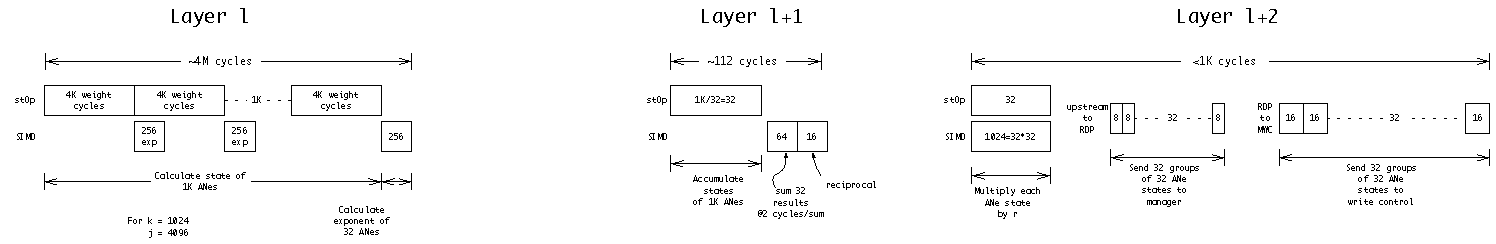
\includegraphics[angle=0, width=1\linewidth]{classifierSequenceTiming}}
      }
      \caption{Classifier layer stOp/SIMD sequence timing}
      \label{fig:classifier implementation sequence timing}
    \end{minipage}
  \end{figure}
  %\vfill
\end{landscape}
\restoregeometry
\newgeometry{letterpaper,top=1in,bottom=1in,right=1in,left=1.25in,footskip=\chapterfootskip, includefoot}
\pagestyle{plain}
\thispagestyle{plain}

